\documentclass{standalone}
\usepackage{tikz}
\usetikzlibrary{patterns, positioning}
\usepackage[sfdefault]{ClearSans} %% option 'sfdefault' activates Clear Sans as the default text font
\usepackage[T1]{fontenc}

\begin{document}
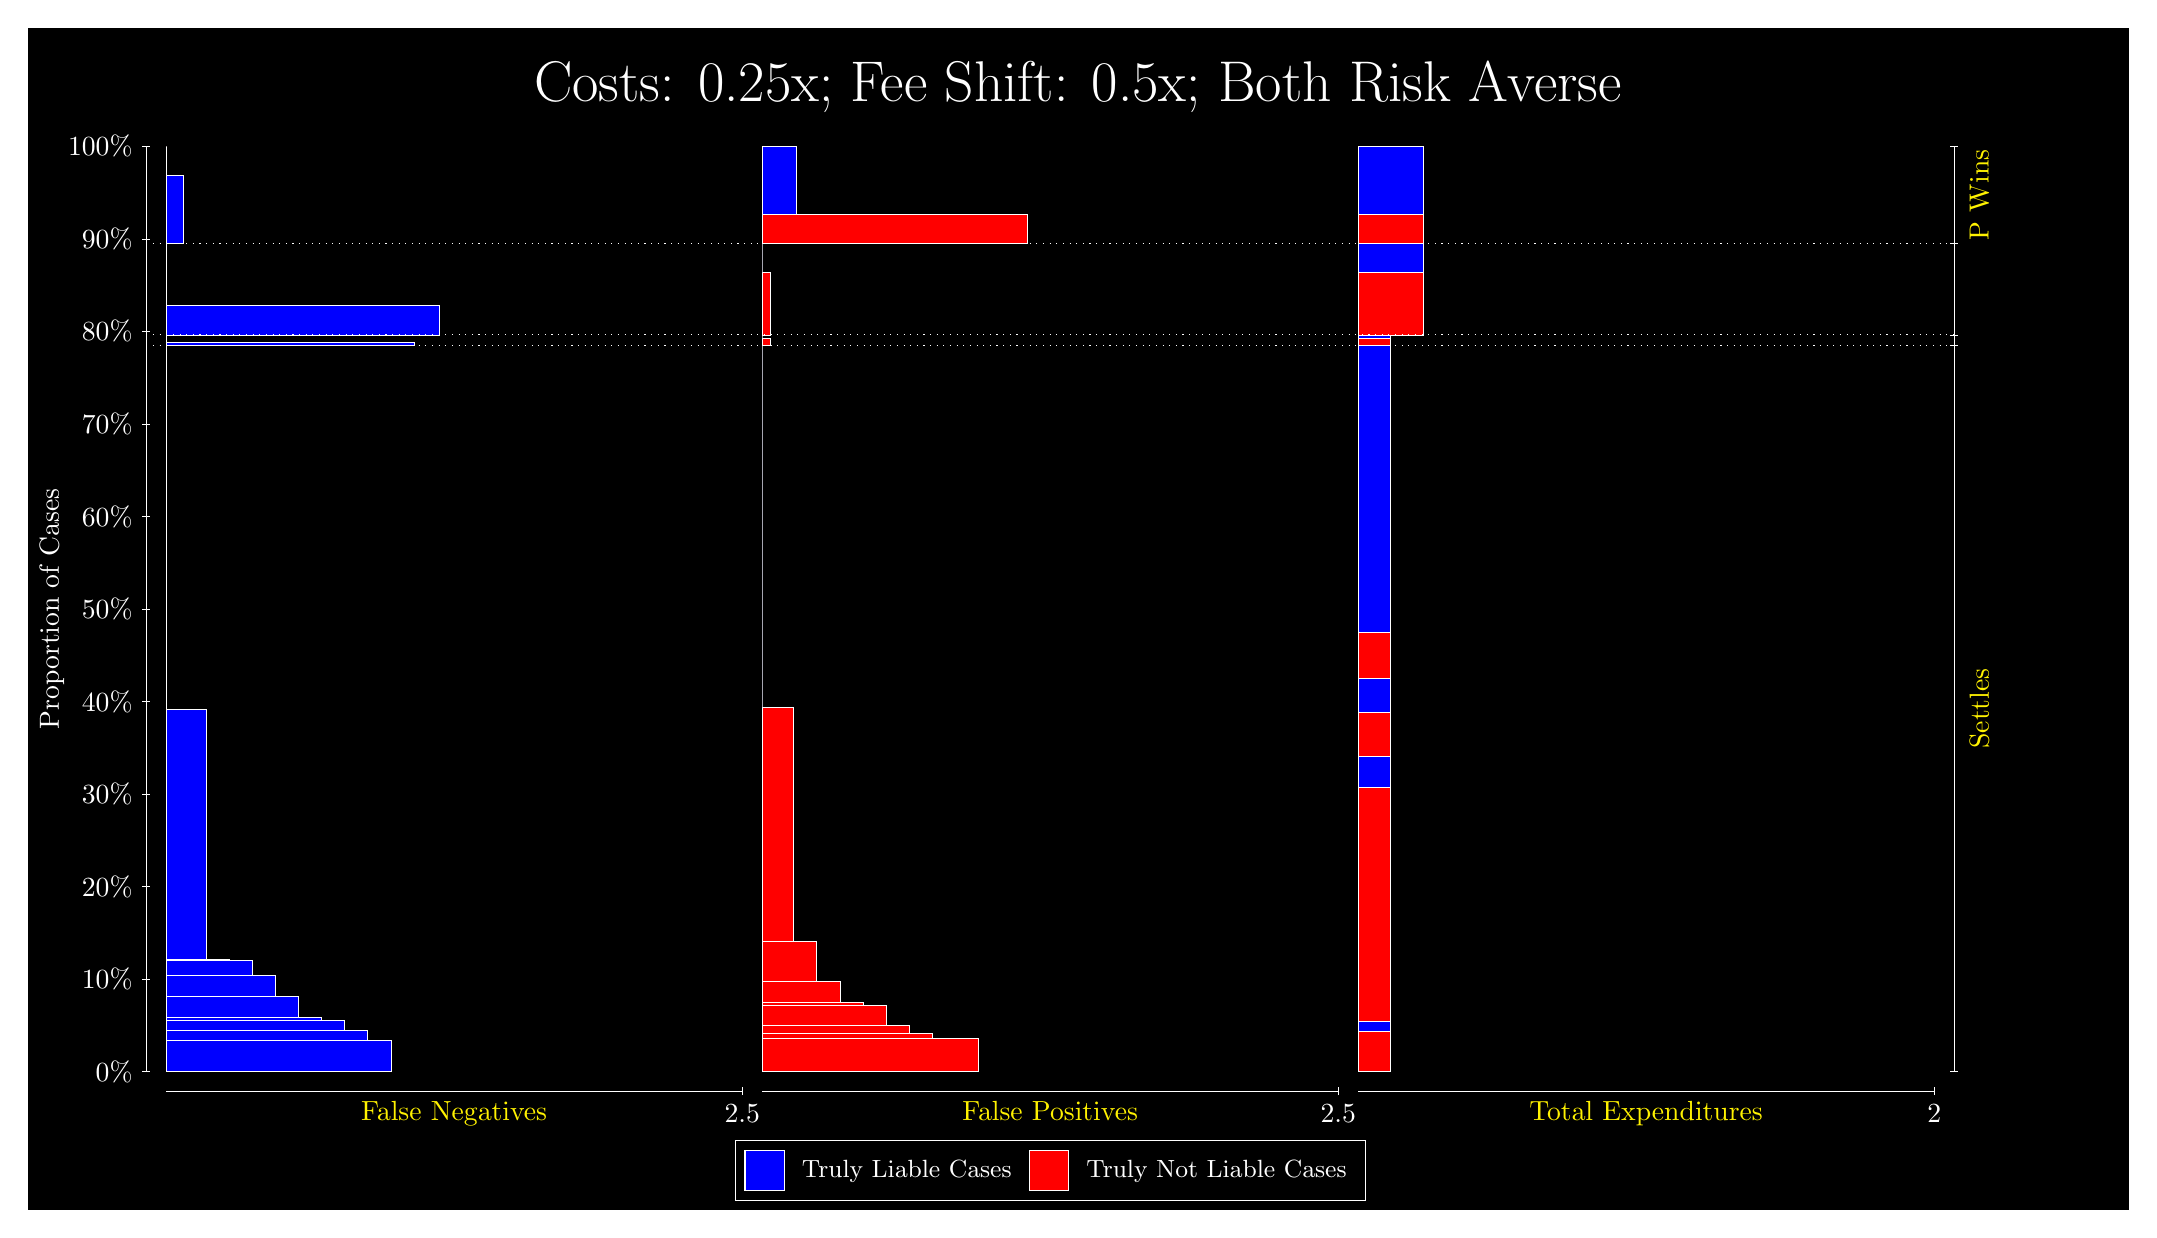
\begin{tikzpicture}
\draw[fill=black] (0,0) rectangle (26.667,15);
\draw[text=white] (0,13.5) rectangle (26.667,15) node[midway] {\huge Costs: 0.25x; Fee Shift: 0.5x; Both Risk Averse};
\draw[white, very thin] (1.5,1.75) -- (1.5,13.5);
\node[rotate=90, text=white, anchor=center] at (0.3, 7.625) {Proportion of Cases};
\draw[white, very thin] (1.45,1.75) -- (1.55,1.75);
\node[text=white, anchor=east] at (1.45, 1.75) {0\%};
\draw[white, very thin] (1.45,2.925) -- (1.55,2.925);
\node[text=white, anchor=east] at (1.45, 2.925) {10\%};
\draw[white, very thin] (1.45,4.1) -- (1.55,4.1);
\node[text=white, anchor=east] at (1.45, 4.1) {20\%};
\draw[white, very thin] (1.45,5.275) -- (1.55,5.275);
\node[text=white, anchor=east] at (1.45, 5.275) {30\%};
\draw[white, very thin] (1.45,6.45) -- (1.55,6.45);
\node[text=white, anchor=east] at (1.45, 6.45) {40\%};
\draw[white, very thin] (1.45,7.625) -- (1.55,7.625);
\node[text=white, anchor=east] at (1.45, 7.625) {50\%};
\draw[white, very thin] (1.45,8.8) -- (1.55,8.8);
\node[text=white, anchor=east] at (1.45, 8.8) {60\%};
\draw[white, very thin] (1.45,9.975) -- (1.55,9.975);
\node[text=white, anchor=east] at (1.45, 9.975) {70\%};
\draw[white, very thin] (1.45,11.15) -- (1.55,11.15);
\node[text=white, anchor=east] at (1.45, 11.15) {80\%};
\draw[white, very thin] (1.45,12.325) -- (1.55,12.325);
\node[text=white, anchor=east] at (1.45, 12.325) {90\%};
\draw[white, very thin] (1.45,13.5) -- (1.55,13.5);
\node[text=white, anchor=east] at (1.45, 13.5) {100\%};

\draw[white, very thin] (24.457,1.75) -- (24.457,13.5);
\draw[white, very thin] (24.407,1.75) -- (24.507,1.75);
\node[anchor=west] at (24.407, 1.75) {};
\draw[white, very thin] (24.407,10.971) -- (24.507,10.971);
\node[anchor=west] at (24.407, 10.971) {};
\draw[white, very thin] (24.407,11.106) -- (24.507,11.106);
\node[anchor=west] at (24.407, 11.106) {};
\draw[white, very thin] (24.407,12.268) -- (24.507,12.268);
\node[anchor=west] at (24.407, 12.268) {};
\draw[white, very thin] (24.407,13.5) -- (24.507,13.5);
\node[anchor=west] at (24.407, 13.5) {};

\draw[white, very thin, fill=blue] (1.75,1.75) rectangle (4.6044,2.1487);
\draw[white, very thin, fill=blue] (1.75,2.1487) rectangle (4.3116,2.2755);
\draw[white, very thin, fill=blue] (1.75,2.2755) rectangle (4.0188,2.4044);
\draw[white, very thin, fill=blue] (1.75,2.4044) rectangle (3.7261,2.443);
\draw[white, very thin, fill=blue] (1.75,2.443) rectangle (3.4333,2.7045);
\draw[white, very thin, fill=blue] (1.75,2.7045) rectangle (3.1406,2.9664);
\draw[white, very thin, fill=blue] (1.75,2.9664) rectangle (2.8478,3.1646);
\draw[white, very thin, fill=blue] (1.75,3.1646) rectangle (2.5551,3.1751);
\draw[white, very thin, fill=blue] (1.75,3.1751) rectangle (2.2623,6.3481);
\draw[white, very thin, fill=red] (1.75,6.3481) rectangle (1.75,10.971);
\draw[white, very thin, fill=blue] (1.75,10.971) rectangle (4.8971,11.016);
\draw[white, very thin, fill=red] (1.75,11.016) rectangle (1.75,11.106);
\draw[white, very thin, fill=blue] (1.75,11.106) rectangle (5.2265,11.479);
\draw[white, very thin, fill=red] (1.75,11.479) rectangle (1.75,12.268);
\draw[white, very thin, fill=blue] (1.75,12.268) rectangle (1.9696,13.127);
\draw[white, very thin, fill=red] (1.75,13.127) rectangle (1.75,13.5);
\draw[white, very thin, fill=red] (9.3189,1.75) rectangle (12.063,2.1662);
\draw[white, very thin, fill=red] (9.3189,2.1662) rectangle (11.771,2.1699);
\draw[white, very thin, fill=red] (9.3189,2.1699) rectangle (11.478,2.2394);
\draw[white, very thin, fill=red] (9.3189,2.2394) rectangle (11.185,2.3313);
\draw[white, very thin, fill=red] (9.3189,2.3313) rectangle (10.892,2.5851);
\draw[white, very thin, fill=red] (9.3189,2.5851) rectangle (10.6,2.6237);
\draw[white, very thin, fill=red] (9.3189,2.6237) rectangle (10.307,2.8956);
\draw[white, very thin, fill=red] (9.3189,2.8956) rectangle (10.014,3.4074);
\draw[white, very thin, fill=red] (9.3189,3.4074) rectangle (9.7214,6.3727);
\draw[white, very thin, fill=blue] (9.3189,6.3727) rectangle (9.3189,10.971);
\draw[white, very thin, fill=red] (9.3189,10.971) rectangle (9.4287,11.061);
\draw[white, very thin, fill=blue] (9.3189,11.061) rectangle (9.3189,11.106);
\draw[white, very thin, fill=red] (9.3189,11.106) rectangle (9.4287,11.895);
\draw[white, very thin, fill=blue] (9.3189,11.895) rectangle (9.3189,12.268);
\draw[white, very thin, fill=red] (9.3189,12.268) rectangle (12.686,12.641);
\draw[white, very thin, fill=blue] (9.3189,12.641) rectangle (9.758,13.5);
\draw[white, very thin, fill=red] (16.888,1.75) rectangle (17.299,2.2619);
\draw[white, very thin, fill=blue] (16.888,2.2619) rectangle (17.299,2.3886);
\draw[white, very thin, fill=red] (16.888,2.3886) rectangle (17.299,5.3539);
\draw[white, very thin, fill=blue] (16.888,5.3539) rectangle (17.299,5.7526);
\draw[white, very thin, fill=red] (16.888,5.7526) rectangle (17.299,6.3169);
\draw[white, very thin, fill=blue] (16.888,6.3169) rectangle (17.299,6.7459);
\draw[white, very thin, fill=red] (16.888,6.7459) rectangle (17.299,7.3271);
\draw[white, very thin, fill=blue] (16.888,7.3271) rectangle (17.299,10.971);
\draw[white, very thin, fill=red] (16.888,10.971) rectangle (17.299,11.061);
\draw[white, very thin, fill=blue] (16.888,11.061) rectangle (17.299,11.106);
\draw[white, very thin, fill=red] (16.888,11.106) rectangle (17.711,11.895);
\draw[white, very thin, fill=blue] (16.888,11.895) rectangle (17.711,12.268);
\draw[white, very thin, fill=red] (16.888,12.268) rectangle (17.711,12.641);
\draw[white, very thin, fill=blue] (16.888,12.641) rectangle (17.711,13.5);
\draw[white, dotted] (1.5,10.971) -- (24.457,10.971);
\draw[white, dotted] (1.5,11.106) -- (24.457,11.106);
\draw[white, dotted] (1.5,12.268) -- (24.457,12.268);
\draw[white, very thin] (1.75,1.5) -- (9.0689,1.5);
\node[text=yellow, anchor=north] at (5.4094, 1.5) {False Negatives};
\draw[white, very thin] (9.0689,1.45) -- (9.0689,1.55);
\node[text=white, anchor=north] at (9.0689, 1.45) {2.5};

\draw[white, very thin] (9.3189,1.5) -- (16.638,1.5);
\node[text=yellow, anchor=north] at (12.978, 1.5) {False Positives};
\draw[white, very thin] (16.638,1.45) -- (16.638,1.55);
\node[text=white, anchor=north] at (16.638, 1.45) {2.5};

\draw[white, very thin] (16.888,1.5) -- (24.207,1.5);
\node[text=yellow, anchor=north] at (20.547, 1.5) {Total Expenditures};
\draw[white, very thin] (24.207,1.45) -- (24.207,1.55);
\node[text=white, anchor=north] at (24.207, 1.45) {2};

\node[text=yellow, centered, rotate=90] at (24.777, 6.3604) {Settles};


\node[text=yellow, centered, rotate=90] at (24.777, 12.884) {P Wins};

\draw (12.978300999999998,1.5) node[draw=none] (baseCoordinate) {};
\begin{scope}[align=center]
        \matrix[scale=0.5, draw=white, below=0.5cm of baseCoordinate, nodes={draw}, column sep=0.1cm]{
            \node[rectangle, draw, minimum width=0.5cm, minimum height=0.5cm, fill=blue] {}; &
            \node[draw=none, font=\small, text=white] (B) {Truly Liable Cases}; &
            \node[rectangle, draw, minimum width=0.5cm, minimum height=0.5cm, fill=red] {}; &
            \node[draw=none, font=\small, text=white] (B) {Truly Not Liable Cases}; \\
            };
\end{scope}

\end{tikzpicture}
\end{document}